\documentclass[twoside,10pt]{article}
\usepackage{/Users/bradenhoagland/latex/styles/toggles}
%\toggletrue{sectionbreaks}
%\toggletrue{sectionheaders}
\newcommand{\docTitle}{HW 5}
\usepackage{/Users/bradenhoagland/latex/styles/common}
\importStyles{modern}{rainbow}{boxy}

%\renewcommand{\theenumi}{\alph{enumi}}

\begin{document}
%\tableofcontents

% ------------------------------
% 1.138
% ------------------------------
\begin{exer}[1.138]
Putnam problem.
\end{exer}

\begin{figure}[H]
        \centering
        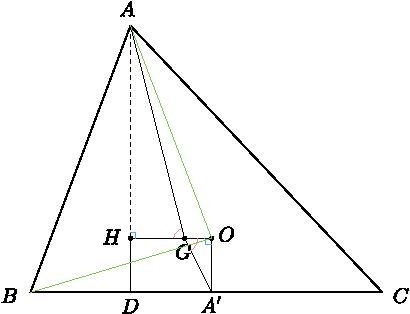
\includegraphics[scale=1]{fig/138.pdf}
        %\caption{}
\end{figure}

By the Euler Line theorem, the centroid $G$ lies on $HO$ and gives the ratio
\[
\frac{|OG|}{|GH|} = \frac{1}{2} .
\] Note that since the two pink angles and the two blue angles are equal, $\Delta AGH \sim \Delta A'GO$. Then we can use the above ratio, along with the given fact $|A'D|=5$, to get
\[
\frac{|A'O|}{|AH|} = \frac{|OG|}{|GH|} \implies |AH| = 10.
\] Then by the Pythagorean Theorem, $|AO|^2 = |AH|^2 + |HO|^2 = 221$. Since $O$ is the circumcenter, $|AO|=|BO|$. Then by the Pythaogrean Theorem again,
\begin{align*}
        |BA'|^2 + |A'O|^2 &= |BO|^2 \\
        |BA'|^2 + |A'O|^2 &= |AO|^2 \\
        |BA'|^2 + 5^2 &= 221 \\
        |BA'| &= 14.
\end{align*}
Since $A'$ is the midpoint of $ BC$, this implies $|BC|=28$.

\newpage

% ------------------------------
% 1.151
% ------------------------------
\begin{exer}[1.151]
Ptolemy's Theorem.
\end{exer}

\begin{figure}[H]
        \centering
        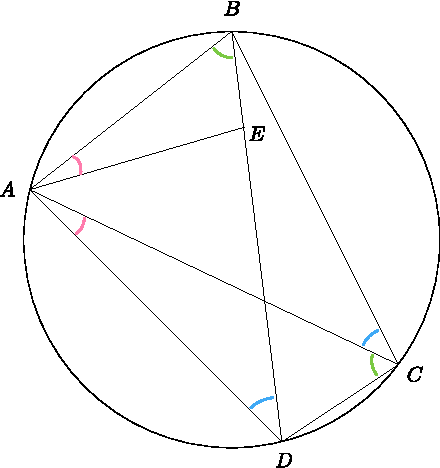
\includegraphics[scale=1]{fig/151.pdf}
        %\caption{}
\end{figure}

Choose $E$ on $BD$ such that $\angle BAE = \angle CAD$. By the Star Trek lemma, since $\angle ABD, \angle ACD$ subtend the same arc, they're equal. Then since they have two equal angles, $\Delta ABE \sim \Delta ACD$. Thus
\[
\frac{|AB|}{|AC|} = \frac{|BE|}{|CD|} \implies |AB| |CD| = |AC| |BE|.
\] Similarly, $\Delta ABC \sim \Delta AED$, so
\[
\frac{|AB|}{|AE|} = \frac{|BC|}{|ED|} \implies |BC| |AD| = |AC| |ED|.
\] Adding these two equalities gives
\begin{align*}
        |AB| |CD| + |BC| |AD| &= |AC| (|BE| + |ED|) \\
                              &= |AC| |DB|.
\end{align*}

\newpage

% ------------------------------
% 1.165
% ------------------------------
\begin{exer}[1.165]
Show $\frac{|\Delta ABP|}{|\Delta APC|} = \frac{|BD|}{|DC|} $, then use this to give an alternative proof of Ceva's Theorem without using Menelaus.
\end{exer}

\begin{figure}[H]
	\centering
	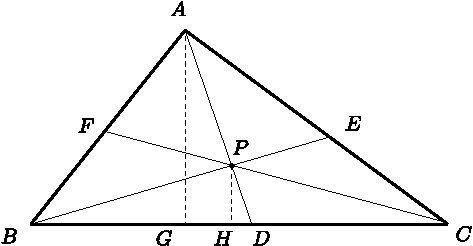
\includegraphics[scale=1]{fig/165.pdf}
	%\caption{}
\end{figure}

\textbf{First part:} Draw the altitudes down from $A$ and $P$ as shown, then we have
\begin{align*}
	|\Delta ABD| &= |\Delta ABP| + |\Delta BPD| \\
	\frac{1}{2} |AG| |BD| &= |\Delta ABP| + \frac{1}{2} |PH| |BD| \\
	\frac{1}{2} |BD| (|AG| - |PH|) &= |\Delta ABP|.
\end{align*}
Similarly, we have
\begin{align*}
	|\Delta ACD| &= |\Delta APC| + |\Delta CDP| \\
	\frac{1}{2} |AG| |DC| &= |\Delta APC| + \frac{1}{2} |PH| |DC| \\
	\frac{1}{2} |DC| (|AG|-|PH|) &= |\Delta APC|.
\end{align*}
Thus their quotient is
\[
\frac{|\Delta ABP|}{|\Delta APC|} = \frac{|BD|}{|DC|} .
\] 

\textbf{Second part:} Using a similar strategy as above, we can show
\[
	\frac{|\Delta APC|}{|\Delta BPC|} = \frac{|AF|}{|FB|} \quad\text{and}\quad \frac{|\Delta BPC|}{|\Delta ABP|} = \frac{|CE|}{|EA|} .
\] Then
\[
\frac{|AF|}{|FB|} \frac{|BD|}{|DC|} \frac{|CE|}{|EA|} = \frac{|\Delta APC|}{|\Delta BPC|} \frac{|\Delta ABP|}{|\Delta APC|} \frac{|\Delta BPC|}{|\Delta ABP|} = 1.
\] The converse direction of Ceva's Theorem from the book requires no change, as it doesn't rely on Menelaus' Theorem.

\newpage

% ------------------------------
% 1.166
% ------------------------------
\begin{exer}[1.166]
Analogue of Menelaus' Theorem when $D$ is at infinity?
\end{exer}

\begin{figure}[H]
	\centering
	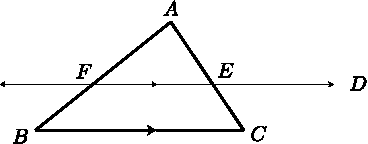
\includegraphics[scale=1.5]{fig/166.pdf}
	%\caption{}
\end{figure}

Note that $D$ is at infinitely if and only if $FE$ is parallel to $BC$. Also note that in this case, we have the signed ratio
\[
	\frac{|BD|}{|DC|} =-1
\] since $D$ is outside of $B$ and $C$. Thus when $D$ is at infinity, Menelaus' theorem becomes
\[
	FE \text{ is parallel to } BC \iff  \frac{|AF|}{|FB|} = \frac{|AE|}{|EC|} .
\] This is precisely Theorem 1.64 in the text, which we've used before.

\newpage

% ------------------------------
% 1.167
% ------------------------------
\begin{exer}[1.167]
Medians intersect at common point.
\end{exer}

\begin{figure}[H]
	\centering
	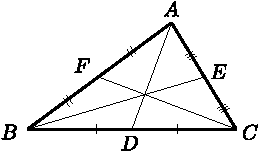
\includegraphics[scale=1.5]{fig/167.pdf}
	%\caption{}
\end{figure}

Since the medians bisect the sides of the $\Delta ABC$,
\[
\frac{|AF|}{|FB|} \frac{|BD|}{|DC|} \frac{|CE|}{|EA|} = 1 \cdot 1 \cdot 1 = 1.
\] Thus by Ceva's theorem, the medians intersect at a common point.

\newpage

% ------------------------------
% 1.168
% ------------------------------
\begin{exer}[1.168]
Altitudes intersect at a common point.
\end{exer}

\begin{figure}[H]
	\centering
	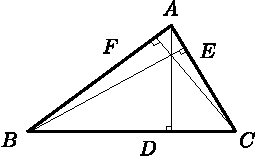
\includegraphics[scale=1.5]{fig/168.pdf}
	%\caption{}
\end{figure}

Since $\Delta BFC$ and $\Delta BDA$ share the angle $\angle ABC$ and since both have a right angle, $\Delta BFC \sim \Delta BDA$. Thus
\[
\frac{|BD|}{|FB|} = \frac{|AB|}{|BC|} .
\] Similarly, $\Delta AFC \sim \Delta AEB$ and $\Delta CDA \sim \Delta CEB$, so
\[
	\frac{|AF|}{|EA|} = \frac{|AC|}{|AB|} \quad\text{and}\quad \frac{|CE|}{|DC|} = \frac{|BC|}{|AC|} .
\] Thus
\[
	\frac{|AF|}{|FB|} \frac{|BD|}{|DC|} \frac{|CE|}{|EA|} = \frac{|AC|}{|AB|} \frac{|AB|}{|BC|} \frac{|BC|}{|AC|} = 1,
\] so by Ceva's theorem, the altitudes intersect at a common point. 

\newpage

% ------------------------------
% 1.169
% ------------------------------
\begin{exer}[1.169]
Angle bisectors intersect at a social point.
\end{exer}

\begin{figure}[H]
	\centering
	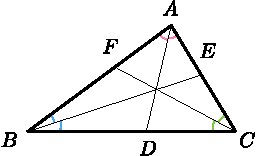
\includegraphics[scale=1.5]{fig/169.pdf}
	%\caption{}
\end{figure}

In Homework 2 we proved the angle bisector theorem, which gives
\[
	\frac{|BD|}{|DC|} = \frac{|AB|}{|AC|} , \qquad \frac{|CE|}{|EA|} = \frac{|BC|}{|AB|} , \quad\text{and} \quad \frac{|AF|}{|FB|} = \frac{|AC|}{|BC|} .
\] Thus
\[
	\frac{|AF|}{|FB|} \frac{|BD|}{|DC|} \frac{|CE|}{|EA|} = \frac{|AC|}{|BC|} \frac{|AB|}{|AC|} \frac{|BC|}{|AB|} = 1,
\] so by Ceva's theorem, the angle bisectors intersect at a common point.

\newpage

\end{document}
